\documentclass[a4paper, 11pt, raggedright, parskip]{tufte-style-article}
% 	class avaliable at:
%	https://github.com/sylvain-kern/tufte-style-article
%

\usepackage{lipsum}


\title{\sffamily\textls{\MakeUppercase{{\Huge Procedure}\\\vskip10pt to plot mass spectroscopy and thermogravimetry data from Netzsch Dispsav and Proteus in Origin software}}}
\author{Sylvain Kern}


\begin{document}

\thispagestyle{empty}
\maketitle
\hfill

This is a guide to process and plot the mass spectroscopy (MS) and thermogravimetry (TG) data recorded from the Netzsch pieces of equipment in Origin 2016 software.\marginnote{Origin 2016 - \url{https://www.originlab.com/index.aspx?go=PRODUCTS/Origin}} This also includes some scripts to automate the process.


All source files can be found at \url{...} along with this very procedure in \texttt{.pdf} or \texttt{.md} formats for user convenience.

\vfill

\begin{center}

\includegraphics[width=.6\textwidth]{figures/Origin8_Logo.png}

\vfill

\includegraphics[width=.8\textwidth]{img_illustration/ms plot example.png}	

\end{center}


\thispagestyle{plain}
\tableofcontents


\newpage
\section{Manual procedure}
\label{sec:full_procedure}

Here is a way to quickly\marginnote{The manual procedure is actually quite long and repetitive, so there is an Origin script presented in section \ref{sec:origin_scripting}.} get \textls{TGMS} plots from data collected in the different Netzsch pieces of software, using Origin.

\margintext {This is a visual overview of the procedure explained below.}%
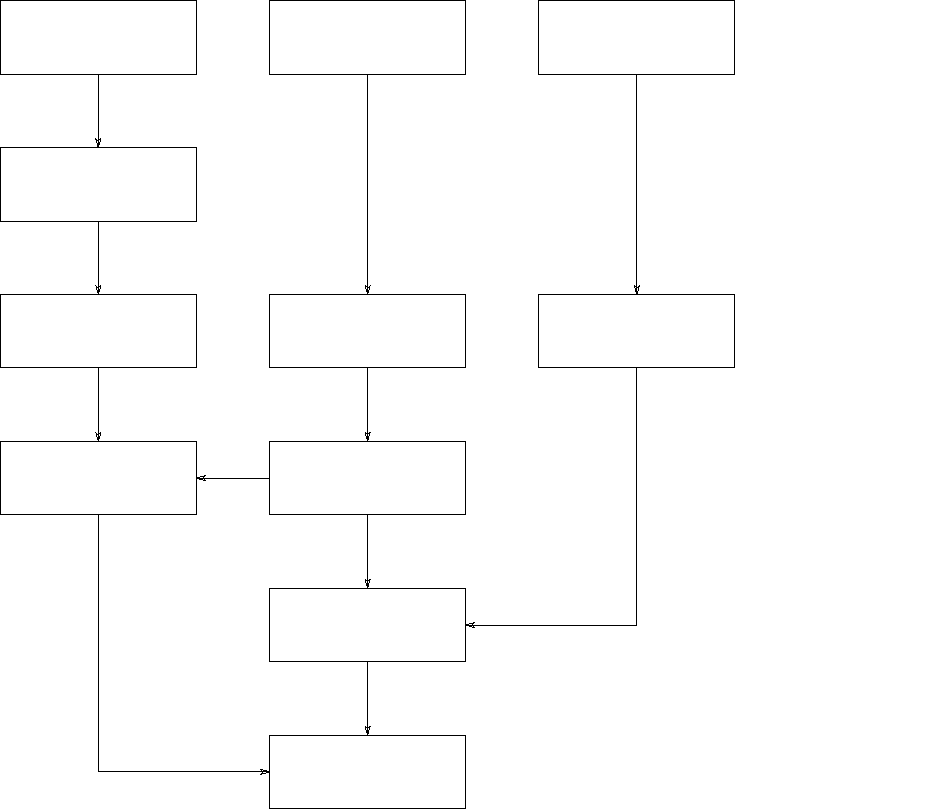
\includegraphics[width=\textwidth]{figures/overview.png}

%\widefig{figures/bliss.jpg}{Blissomaxxouillamosse}{fig:bliss}


\subsection{Exports}


\subsubsection{Export MS data from  Dispsav}

\begin{enumerate}
	
\item Open Aëolos Dispsav.

\item Go to the \texttt{Process} tab, go to \texttt{Cycles...} and open the desired \texttt{.mdc}.

\item Then go to \texttt{File > Convert to ASCII...}. 

\item Save the \texttt{.asc} file into a chosen folder.

\item Open this \texttt{.asc} file with a notepad and note the number of points and the maximum time, which appear in the header lines or in the last line of the two firsts columns.

\end{enumerate}


\subsubsection{Export TG data form Netzsch Proteus}

\begin{enumerate}
	
\item Open Proteus Analysis.
	
\item Go to \texttt{File > Open...} and open the \texttt{.ngb-ss1} file of your choice.

\item Then go to \texttt{Extras > Export Data...}. Choose the range and number of points\marginnote{Since the TG and MS experiments have been made at the same time with the same temperature increase, the temperature measurements and the step should match for the MS and TG.}. The number of points must be exactly the same as in the \texttt{.asc} file exported from Dispsav. Check that the maximum time matches too.

\end{enumerate}


\subsubsection{Export baseline data}

The baseline data is in the same form than the TG data, so the steps are exacly similar than those on the paragraph above. Again, export it with exactly the same number of points and maximum time as in the MS.


\subsection{Imports in Origin}

\margintext{This procedure has been made using Origin 2016 version 93E. The software may differ a bit if you use more recent versions of the software. For more help, see Origin's user guide: \url{www.originlab.com/doc/User-Guide}}The data treatments will be executed on Origin software. To continue, open Origin.


\subsubsection{Import MS data in ASCII format}

Here are the steps to import the first MS data worksheet, \textit{i.e} the relative intensity extrema for each $M/z$.

\begin{enumerate}

\item On Origin, go to \texttt{File > Import > Import Wizard} or press \texttt{Ctrl+3}.
\margintext{If the \texttt{Import} line does not appear on the \texttt{File} menu, make sure an Origin project is open by clicking \texttt{File > New > Project}.}

\item On the \texttt{Import Wizard - Source} window, select the MS data file you saved. Make sur the data type ASCII is selected, and click \texttt{Next}.

\includegraphics[width=.8\textwidth]{figures/import ms/source_1.png}

\item On the \texttt{Import Wizard - Header Lines} window, specify the number of header lines --\textit{i.e.} the number of lines which will be ignored by Origin. Leave the \texttt{Number of subheader lines} at \texttt{0}, and \texttt{Long Names} at \texttt{0} too.

\includegraphics[width=.8\textwidth]{figures/import ms/header_lines_1.png}

The data preview should look like this: header lines in  black and data lines in gray.

Then, click \texttt{Next}.

\item On \texttt{Variable Extraction} window, verify that the \texttt{Save file into a workbook} box is ticked. Leave the other boxes blank and click \texttt{Next}. 

\includegraphics[width=.8\textwidth]{figures/import ms/variable_extraction_1.png}

\item On \texttt{File name options}, tick the \texttt{Worksheet with filename} box and leave the others alone. Then go \texttt{Next}.

\includegraphics[width=.8\textwidth]{figures/import ms/file_name_options_1.png}

\item On \texttt{Data Columns}, select the number of columns there are in the imported file, -- here 6, click \texttt{Apply} and make sure that the data is properly formatted in the preview window. Select the \texttt{1,000.00} numeric separator and go to the \texttt{Next} page.

\includegraphics[width=.8\textwidth]{figures/import ms/data_columns_1.png}

\item On \texttt{Data Selection}, just leave \texttt{Partial import} to \texttt{None} click \texttt{Next} --~the data should be correctly displayed in the window below, just like in the last step. Then go \texttt{Next}.

\includegraphics[width=.8\textwidth]{figures/import ms/data_selection_1.png}

\item On \texttt{Save Filters}, leave everything as it is, unless you want to save this import filter for a next time. Click \texttt{Finish}.

\end{enumerate}

\newpage

Now your worksheet should look like this:\marginnote{It is possible that Origin creates another empty worksheet with the same name as the one you created, and I don't know why. You can just delete it by right-clicking on it \texttt{> Delete}.}

\includegraphics[width=\textwidth]{figures/import ms/data_preview_1.png}



To import the second MS piece of data, see the following steps.

\begin{enumerate}

\item Create a new worksheet by right-clicking a worksheet tab on the bottom, "\texttt{Add}".

\item Open \texttt{File > Import > Import Wizard} or press \texttt{Ctrl+3}.

\item On the \texttt{Import Wizard - Source} window, select the MS data file you saved. Make sur the data type ASCII is selected, and click \texttt{Next}.

\item On the \texttt{Import Wizard - Header Lines} window, specify the number of header lines --\textit{i.e.} the number of lines which will be ignored by Origin. This time, put the \texttt{Number of subheader lines} at 1, and \texttt{Long Names} at 1 too.

\includegraphics[width=.8\textwidth]{figures/import ms/header_lines_2.png}

The data preview should look like this, with the subheader lines highlighted in blue.

Then, click \texttt{Next}.

\item On \texttt{Variable Extraction} window, verify that the \texttt{Save file into a workbook} box is ticked. Leave the other boxes blank and click \texttt{Next}. 

\item On \texttt{File name options}, tick the \texttt{Worksheet with filename} box and leave the others alone. Then go \texttt{Next}.

\item On \texttt{Data Columns}, select the number of columns there are in the imported file, -- here 25, click \texttt{Apply} and make sure that the data is properly formatted in the preview window. Select the \texttt{1,000.00} numeric separator and go to the \texttt{Next} page.

\includegraphics[width=.8\textwidth]{figures/import ms/data_columns_2.png}

\item On \texttt{Data Selection}, just leave \texttt{Partial import} to \texttt{None} and click \texttt{Next} --~the data should be correctly displayed in the window below, just like in the last step. Then go \texttt{Next}.

\includegraphics[width=.8\textwidth]{figures/import ms/data_selection_2.png}

\item On \texttt{Save Filters}, leave everything as it is, unless you want to save this import filter for a next time. Click \texttt{Finish}.

\end{enumerate}

Your second worksheet should look like this.

Now you have two worksheets, one with $M/z$ data, the other with the actual MS curves.

To make future worksheet reference easier, I renamed the worksheets with the respective names "\texttt{mz sheet}", "\texttt{ms data}". To do the same, right-click a worksheet tab on the bottom, "\texttt{Name and Comments...}" and fill the "\texttt{Short Name}" field.

\includegraphics[width=.5\textwidth]{figures/import ms/renamed.png}

\smallskip

\begin{wide}
\includegraphics[height=200pt]{figures/import ms/data_preview_1.png}
\hfill
\includegraphics[height=200pt]{figures/import ms/data_preview_2.png}
\end{wide}

\subsubsection{Import TG data in \texttt{.txt} format}
\label{subsubsec:import_tg}

This is a bit shorter than the MS import but it is the same idea.

\begin{enumerate}

\item Create a new worksheet and switch to it.

\item Reach \texttt{File > Import > Import Wizard} and browse the desired file.

\item Plot 

\end{enumerate}	


\subsubsection{Import baseline data in \texttt{.txt} format}

The steps are the same than the TG import in paragraph \ref{subsubsec:import_tg} since the files are formatted in the same way.


\subsection{Preliminary treatments}

You can rearrange the columns of your worksheets the way you want, delete some of the useless information, put names, units, comments etc\dots{}

sThe following steps treat the data to prepare the TGMS plots.


\subsection{Place the $M/z$ labels on MS columns}


\subsection{Calculate the relative intensity on mz sheet}


\subsubsection{Polynomial regression of the temperature curve in TG data}

\margintext{The fit must only consider the points where the temperature grows --~approximately~-- linearly, therefore it must omit all points from segment 2 and 3. The temperature increase shows some variations at the beginning, until a stabilized growth settles. Usually, this variation becomes marginal around $T = 200 \text{ °C}$.}
Since temperature \textit{vs.} time is not given in the MS data, it is needed to whether fit a curve, whether interpolate the data, to get new temperature points corresponding to MS time points.
 
Assuming the {\lsstyle PID} controller for the furnace is well adjusted, the temperature increase in the furnace should be linear so I chose to fit a degree one polynomial in this case.


\subsubsection[Baseline mass loss data interpolation and substraction]{Baseline mass loss data interpolation and substraction\marginnote{This is only needed if the TG and baseline data don't have the same measurement points. If they have been exported from Proteus with the same settings, please ignore this part.}}

The time points for TG and baseline may not be the same. If it is the case, we will want to interpolate the baseline mass loss data in order to get the correct values to substract from TG ones, since the baseline data does not follow a predictable model.


\subsection{Plotting graphs}


\subsubsection{For TG}


\subsubsection{For MS}


\subsubsection{Plot TGMS graph}


\section{Origin scripting for automated plots}
\label{sec:origin_scripting}	
	
To reduce the time spent on overly repetitive tasks, I produced a LabTalk -- Origin's scripting language -- file run by Origin to execute the procedure detailed above in section \ref{sec:full_procedure}.


\subsection{Scripts installation}

Go to the following address:

\noindent\url{https://github.com/sylvain-kern/tgmsplot-script}

\noindent and reach for the \inlinecode{text}{setup.exe} file in the \texttt{setup} folder. Download it and run it\marginnote{Do not worry if Windows freaks out and thinks it is a virus, I do not have an authentification certificate indeed, so I can not guarantee to Windows that my program is safe.}. The setup creates a \texttt{tgmsplot-script} folder in the Origin files directory a and puts the script files in it. When installing, verify the destination folder, by default it is
\begin{codebox}{text}
C:\Program Files\OriginLab\Origin2016
\end{codebox}
but it can change with your version of Origin.


\littletitle{Manual installation}
Download the folder that contains the source files on the project repository:

\noindent\url{https://github.com/sylvain-kern/tgmsplot-script}.

Place the \texttt{tgmsplot-script} in the following folder:

\margintext{If you have a different version of Origin, it may not be '\texttt{...$\backslash$Origin2016}' but whatever your version is.}%
\begin{codebox}{text}
C:\ProgramFiles\Origin2016\
\end{codebox}

\littletitle{Button groups}
On Origin, go to \texttt{View > Toolbars} or press \texttt{Ctrl+T}. Go to the \texttt{Button groups} tab

\subsection{Usage}

\littletitle{Using buttons}

i n s t a l l   b u t t o n s

\littletitle{Using the \texttt{run.file} command}
Open the command window --this icon \includegraphics[height=12pt]{figures/command window.png} on the right of the top toolbar. Then run the following command:

\begin{codebox}{text}
run.file("C:\ProgramFiles\Origin2016\tgmsplot-script\<file>")
\end{codebox}

A file browser window appears, select the file you want to load.

To import only the MS data, run the following in the command window:\marginnote{Note that the scipt will \textls{NOT} work if the file name contains accents or fancy characters.} you wand to load. Click \texttt{Ok} then do the same for the TG and baseline files.\margintext{The MS curves are not to scale on the $y$ axis, which is not ticked. The TGMS plot is only meant to give a qualitative overview and not precise quantitative information.}
\begin{codebox}{text}
run.file("C:\Program Files\Origin2016\tgmsplot-script\import-ms.ogs")
\end{codebox}
The same goes for TG and BL data:
\begin{codebox}{text}
run.file("C:\Program Files\Origin2016\tgmsplot-script\import-tg.ogs")
\end{codebox}
\begin{codebox}{text}
run.file("C:\Program Files\Origin2016\tgmsplot-script\import-bl.ogs")
\end{codebox}
Then, execute the plot program:
\begin{codebox}{text}
run.file("C:\Program Files\Origin2016\tgmsplot-script\plot.ogs")
\end{codebox}


\subsubsection{Script and execution details}

The source folder contains the following files:

\begin{wide}
\begingroup
\centering
\renewcommand*{\arraystretch}{1.5}
\begin{tabularx}{.8\linewidth}{rX}
\inlinecode{text}{import-ms.ogs}		& imports MS data, whether from 'regular' or bargraph formattings;\\
\inlinecode{text}{import-tg.ogs}		& imports tg data;\\
\inlinecode{text}{plot-vs-temp}		& plots chosen data \textit{vs.} temperature;\\
\inlinecode{text}{plot-vs-time}		& plots chosen data \textit{vs.} time;\\
\end{tabularx}
\endgroup
\end{wide}

I recommend using \texttt{main.ogs} rather than the individual separate files, as some dependency issues may appear.


\subsubsection{Button groups}

i n   p r o g r e s s

create new project unlocks access to the buttons


\subsection{Issues}

i n   p r o g r e s s

Bargraph data format not supported. \textsc{it is now}!










\end{document}